\documentclass{standalone}
\usepackage{tikz}
\begin{document}
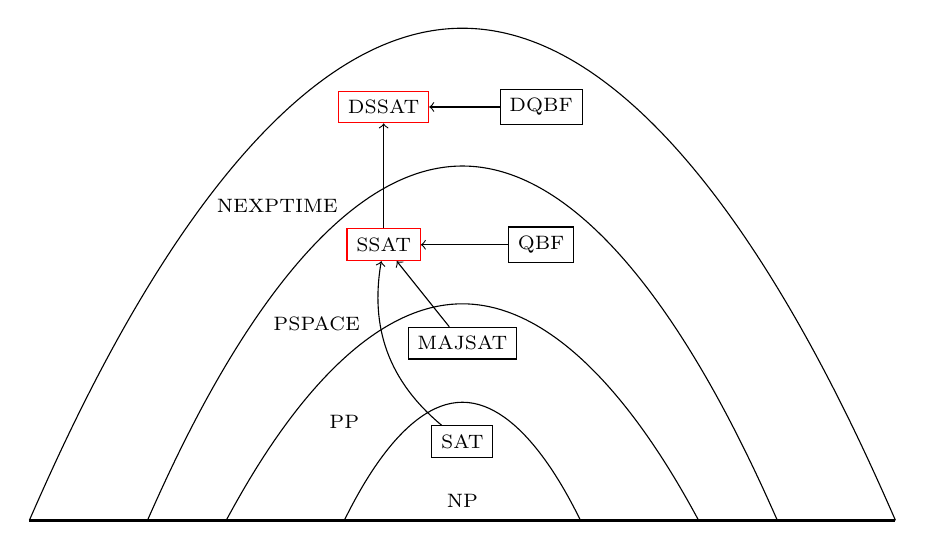
\begin{tikzpicture}[auto]
    \tikzstyle{every node}=[font=\scriptsize]
    \pgftransformscale{.5}
    %%% HELP LINES - uncomment to design/extend
    %\draw[step=1cm,gray,very thin] (-10,0) grid (10,12);
    %\node at (0,0) {\textbf{(0,0)}};
    %% Horizontal bar
    \draw[very thick] (-11,0) -- (11,0);
    % NP
    \draw (-3,0) parabola bend (0,3) (3,0);
    \node at (0,0.5) {NP};
    \node at (0,2) [draw,rectangle] (SAT) {SAT};
    % PP
    \draw (-6,0) parabola bend (0,5.5) (6,0);
    \node at (-3,2.5) {PP};
    \node at (0,4.5) [draw,rectangle] (MAJSAT) {MAJSAT};
    % PSPACE
    \draw (-8,0) parabola bend (0,9) (8,0);
    \node at (-3.7,5) {PSPACE};
    \node at (2,7) [draw,rectangle] (QBF) {QBF};
    \node at (-2,7) [draw=red,rectangle] (SSAT) {SSAT};
    % NEXPTIME
    \draw (-11,0) parabola bend (0,12.5) (11,0);
    \node at (-4.7,8) {NEXPTIME};
    \node at (2,10.5) [draw,rectangle] (DQBF) {DQBF};
    \node at (-2,10.5) [draw=red,rectangle] (DSSAT) {DSSAT};

    \path
    (SAT) edge [->,bend left] (SSAT)
    (MAJSAT) edge [->] (SSAT)
    (QBF) edge [->] (SSAT)
    (SSAT) edge [->] (DSSAT)
    (DQBF) edge [->] (DSSAT);
\end{tikzpicture}
\end{document}